\section{Normalizing Flows on Hyperbolic Spaces}
We seek to define flexible and learnable distributions on $\mathbb{H}^n_K$, which will allow us to learn rich approximate posterior distributions for hierarchical data.
To do so, we design a class of invertible parametric hyperbolic functions, $f_i: \mathbb{H}^n_K \to \mathbb{H}^n_K$.
A sample from the approximate posterior can then be obtained by first sampling from a simple base distribution $\mb{z}_0 \sim p(\mb{z})$ defined on $\mathbb{H}^n_K$ and then applying a composition of $f_{i\in[j]}$ functions from this class: $\mb{z}_j = f_j \circ f_{j-1} \circ \dots \circ f_1(\mb{z}_0)$.

In order to ensure effective and tractable learning, the class of functions $f_i$ we define must satisfy three key desiderata:
\begin{enumerate}[itemsep=0pt, parsep=0pt, topsep=0pt]
    \item Each function $f_i$ must be invertible. 
    \item We must be able to efficiently sample from the final distribution, after applying $\mb{z}_j = f_j \circ f_{j-1} \circ \dots \circ f_1(\mb{z}_0)$. 
    \item We must be able to efficiently compute the associated change in volume ---i.e., the Jacobian determinant, of the overall transformation.
\end{enumerate}
 Given these requirements, the final transformed distribution is given by the change of variables rule:
\begin{equation}
    \log p(\mb{z}_j) = \log p(\mb{z}_0) - \sum_{i=1}^k\log \textnormal{det}\Big|\frac{\partial f_j}{\partial z_{j-1}} \Big|.
\end{equation}
\cut{The desiderata 1-3 above ensure that this density is well-defined and efficiently computable.}
Functions satisfying desiderata 1-3 in Euclidean space are often termed {\em normalizing flows} (Appendix \ref{normalizing_flow_appendix}), and our work extends this idea to hyperbolic manifolds. In the following sections we describe two flows of increasing complexity, Tangent Coupling ($\mathcal{T}C$) and Wrapped Hyperboloid Coupling ($\mathcal{W}HC$). The first approach lifts a standard Euclidean flow to the tangent space at the origin of the hyperboloid.
The second approach modifies the flow to explicitly utilize hyperbolic geometry. Figure \ref{fig:density_estimation} illustrates synthetic densities on hyperbolic space learned by our approach.


\subsection{Tangent Coupling}
Similar to the Wrapped Normal distribution (Section \ref{sec:hyperprobs}), one strategy to define a normalizing flow on the hyperboloid is to use the tangent space at the origin. That is, we first sample a point from our base distribution---which we define to be a Wrapped Normal---and use the logarithmic map at the origin to transport it to the corresponding tangent space. Once we arrive at the tangent space we are free to apply any Euclidean flow before finally projecting back to the manifold using the exponential map. 
This approach leverages the fact that the tangent bundle of a hyperbolic manifold has a well-defined vector space structure, allowing affine transformations and other operations that are ill-defined on the manifold itself. 
%the disjoint union of all tangent spaces, \textit{tangent bundle}, of a hyperbolic manifold has a well-defined vector space structure, allowing affine transformations and other operations that are ill-defined on the manifold itself. 

Following this idea, we build upon one of the earliest and most well-studied flows: the RealNVP flow \cite{dinh2016density}. At its core, the RealNVP flow uses a computationally symmetric transformation (affine coupling layer) which has the benefit of being fast to evaluate and invert due to its triangular Jacobian, whose determinant is cheap to compute. Operationally, the coupling layer is implemented using a binary mask, and partitions some input $x$ into two sets, where the first set, $x_1:=x_{0:d}$ is transformed elementwise independently of other dimensions. The second set, $x_2:=x_{d+1:n}$, is also transformed elementwise but in a way that depends on the first set (see Appendix \ref{Euclidean_RealNVP_appendix} for more details). Since all coupling layer operations occur at $\mathcal{T}_{\textbf{o}}\mathbb{H}^n_K$ we term this form of coupling as Tangent Coupling ($\mathcal{T}C$). 

Thus the overall transformation due to one layer of our $\mathcal{T}C$ flow is then a composition of a logarithmic map, affine coupling defined on $\mathcal{T}_{\textbf{o}}\mathbb{H}^n_k$, and an exponential map:
\begin{align}
    \label{eq:tangent_coupling}
     \tilde{f}^{\mathcal{T}C}(\tilde{x}) &=
     \begin{cases}
     \tilde{z}_{1} &= \tilde{x}_{1} \\
     \tilde{z}_{2} &= \tilde{x}_{2} \odot \sigma(s(\tilde{x}_{1})) + t(x_1) \nonumber
     \end{cases}\\
    %f(\tilde{x}) &=  b \odot \tilde{x} + (1 - b)\odot(\tilde{x} \odot \sigma(s(b \odot \tilde{x})) + t(b \odot \tilde{x})) \nonumber \\
    %\textbf{y} =&  \textnormal{exp}_{\textbf{o}}(f(\tilde{x})) ,
    f^{\mathcal{T}C}(\mb{x}) &= \textnormal{exp}_{\textbf{o}}(\tilde{f}^{\mathcal{T}C}(\log_{\textbf{o}}(\textbf{x}))),
\end{align}
where $\tilde{x} = \log_{\textbf{o}}(\textbf{x})$ is a point on $\mathcal{T}_{\textbf{o}}\mathbb{H}^n_K$, and $\sigma$ is a pointwise non-linearity such as the exponential function. Functions $s$ and $t$ are parameterized scale and translation functions implemented as neural nets from $\mathcal{T}_{\textbf{o}}\mathbb{H}^{d}_K \to \mathcal{T}_{\textbf{o}}\mathbb{H}^{n-d}_K$.
One important detail is that arbitrary operations on a tangent vector $v \in \mathcal{T}_{\textbf{o}}\mathbb{H}^n_K$ may transport the resultant vector outside the tangent space, hampering subsequent operations.
To avoid this we can keep the first dimension fixed at $v_0 = 0$ to ensure we remain in $\mathcal{T}_{\textbf{o}}\mathbb{H}^{n}_K$.
\cut{
\begin{align}
    \textbf{y} &=  \textnormal{exp}_{\textbf{o}}(f(\tilde{x})) ,
\end{align}
}

\begin{figure}[t!]
     \centering
     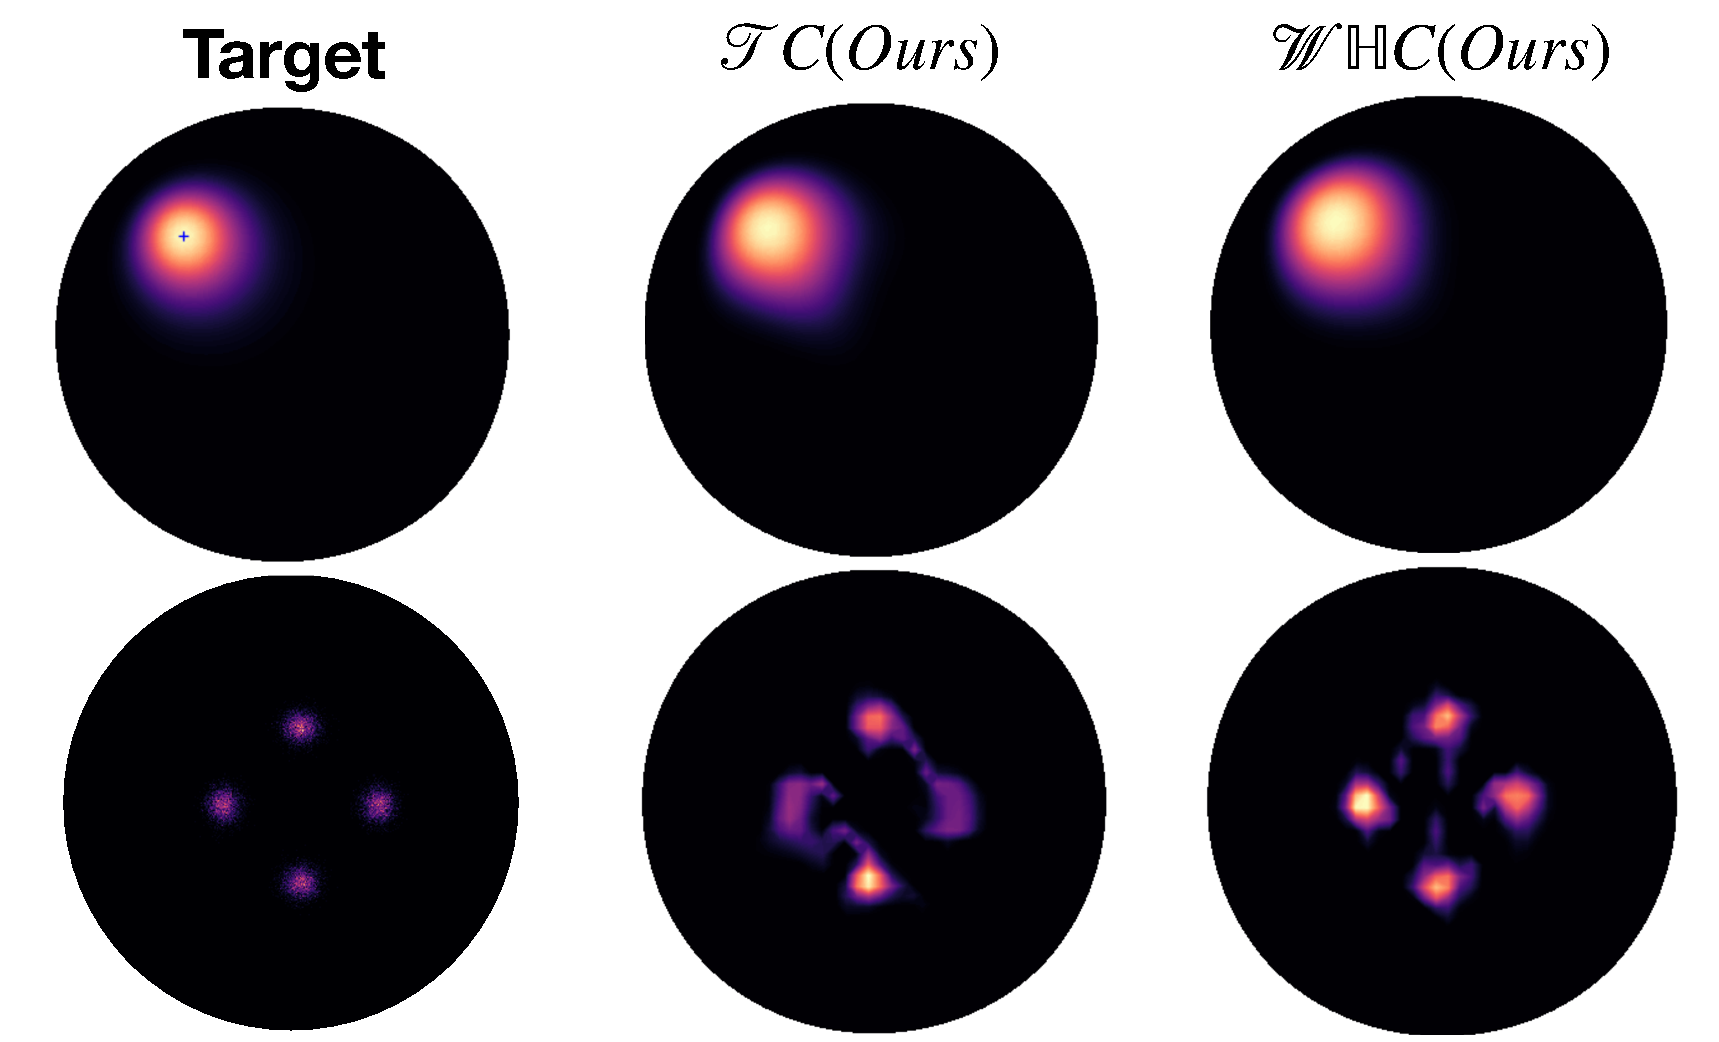
\includegraphics[width=\linewidth]{hyperbolic_density_graphic.pdf}
     \vspace{-10pt}
     \caption{Comparison of density estimation in hyperbolic space for 2D wrapped Gaussian (WG) and mixture of wrapped gaussian (MWG) on $\mathbb{D}^2_1$. Densities are visualized in the Poincare disk.}
     \vspace{-10pt}
     \label{fig:density_estimation}
 \end{figure}

Similar to the Euclidean RealNVP, we need an efficient expression for the Jacobian determinant of $f^{\mathcal{T}C}$.
\begin{prop}
The log Jacobian determinant of a single $\mathcal{T}C$ layer in \eqref{eq:tangent_coupling} is:
\begin{align}
\cut{
    \textnormal{det}\Big (\frac{\partial \textbf{y}}{\partial \textbf{x}}\Big) =  \textnormal{det}\Big (\frac{\partial \textnormal{exp}_{\textbf{o}}(z)}{\partial z}\Big) \cdot \textnormal{det}\Big (\frac{\partial f(\tilde{x})}{\partial \tilde{x}}\Big) \cdot  \textnormal{det}\Big (\frac{\partial \log_{\textbf{o}}(\textbf{x})}{\partial \textbf{x}}\Big)
    }
     \log \textnormal{det}\Big (\frac{\partial \textbf{y}}{\partial \textbf{x}}\Big) &= \Big(\frac{R\sinh(\frac{||z||_{\mathcal{L}}}{R})}{||z||_{\mathcal{L}}}\Big)^{n-1} + \prod_{i=d+1}^n\sigma(s(\tilde{x}_1))_i  \nonumber\\
     & + \Big(\frac{R\sinh(\frac{||\log_{\textbf{o}}(\textbf{x})||_{\mathcal{L}}}{R})}{||\log_{\textbf{o}}(\textbf{x})||_{\mathcal{L}}}\Big)^{1-n}
    %\label{jac_det_tangent_flow_1}.
\end{align}
where, $ \mb{z} =  \tilde{f}^{\mathcal{T}C}(\tilde{x})$ and $\tilde{f}^{\mathcal{T}C}$ is as defined above.
\end{prop}
\begin{proofsketch}
Here we only provide a sketch of the proof and details can be found in Appendix \ref{tangent_coupling_proof_appendix}. First, observe  that the overall transformation  is a valid composition of functions: $\mb{y} := \textnormal{exp}_{\textbf{o}} \circ \tilde{f}^{\mathcal{T}C} \circ \log_{\textbf{o}}(\textbf{x})$. Thus, the overall determinant can be computed by chain rule and the identity,  $\textnormal{det}\Big (\frac{\partial \textbf{y}}{\partial \textbf{x}}\Big) =  \textnormal{det}\Big (\frac{\partial \textnormal{exp}_{\textbf{o}}(z)}{\partial z}\Big) \cdot \textnormal{det}\Big (\frac{\partial f(\tilde{x})}{\partial \tilde{x}}\Big) \cdot  \textnormal{det}\Big (\frac{\partial \log_{\textbf{o}}(\textbf{x})}{\partial \textbf{x}}\Big)$. Tackling each function in the composition individually, $\textnormal{det}\Big (\frac{\partial \textnormal{exp}_{\textbf{o}}(z)}{\partial z}\Big) = \Big(\frac{R\sinh(\frac{||z||_{\mathcal{L}}}{R})}{||z||_{\mathcal{L}}}\Big)^{n-1}$ as derived in \cite{skopek2019mixed}. As the logarithmic map is the inverse of the exponential map the log Jacobian determinant is simply the inverse of the determinant of the exponential map, which gives the $\textnormal{det}\Big (\frac{\partial \log_{\textbf{o}}(\textbf{x})}{\partial \textbf{x}}\Big)$ term. 
For the middle term, we must calculate the directional derivative of $\tilde{f}^{\mathcal{T}C}$ with respect to an orthonormal basis of $\mathcal{T}_{\textbf{o}}\mathbb{H}^{n}_K$. Since the standard Euclidean basis vectors $e_1, ..., e_n$ are also a basis for $\mathcal{T}_{\textbf{o}}\mathbb{H}^{n}_K$, the log Jacobian determinant $\textnormal{det}\Big (\frac{\partial f(\tilde{x})}{\partial \tilde{x}}\Big)$ simplifies to that of the RealNVP flow, is lower triangluar and is thus efficiently computable in $\mathcal{O}(n)$ time.

\end{proofsketch}
It is remarkable that the middle term in Proposition 1 is precisely the same change in volume associated with Euclidean coupling in RealNVP.
The change in volume due to the hyperbolic space only manifests itself through the exponential and logarithmic maps, each of which can be computed in $\mathcal{O}(n)$ cost. Thus, the overall cost is only slightly larger than the regular Euclidean RealNVP, but still $\mathcal{O}(n)$.



\subsection{Wrapped Hyperboloid Coupling}
\begin{figure}[ht]
    \centering
    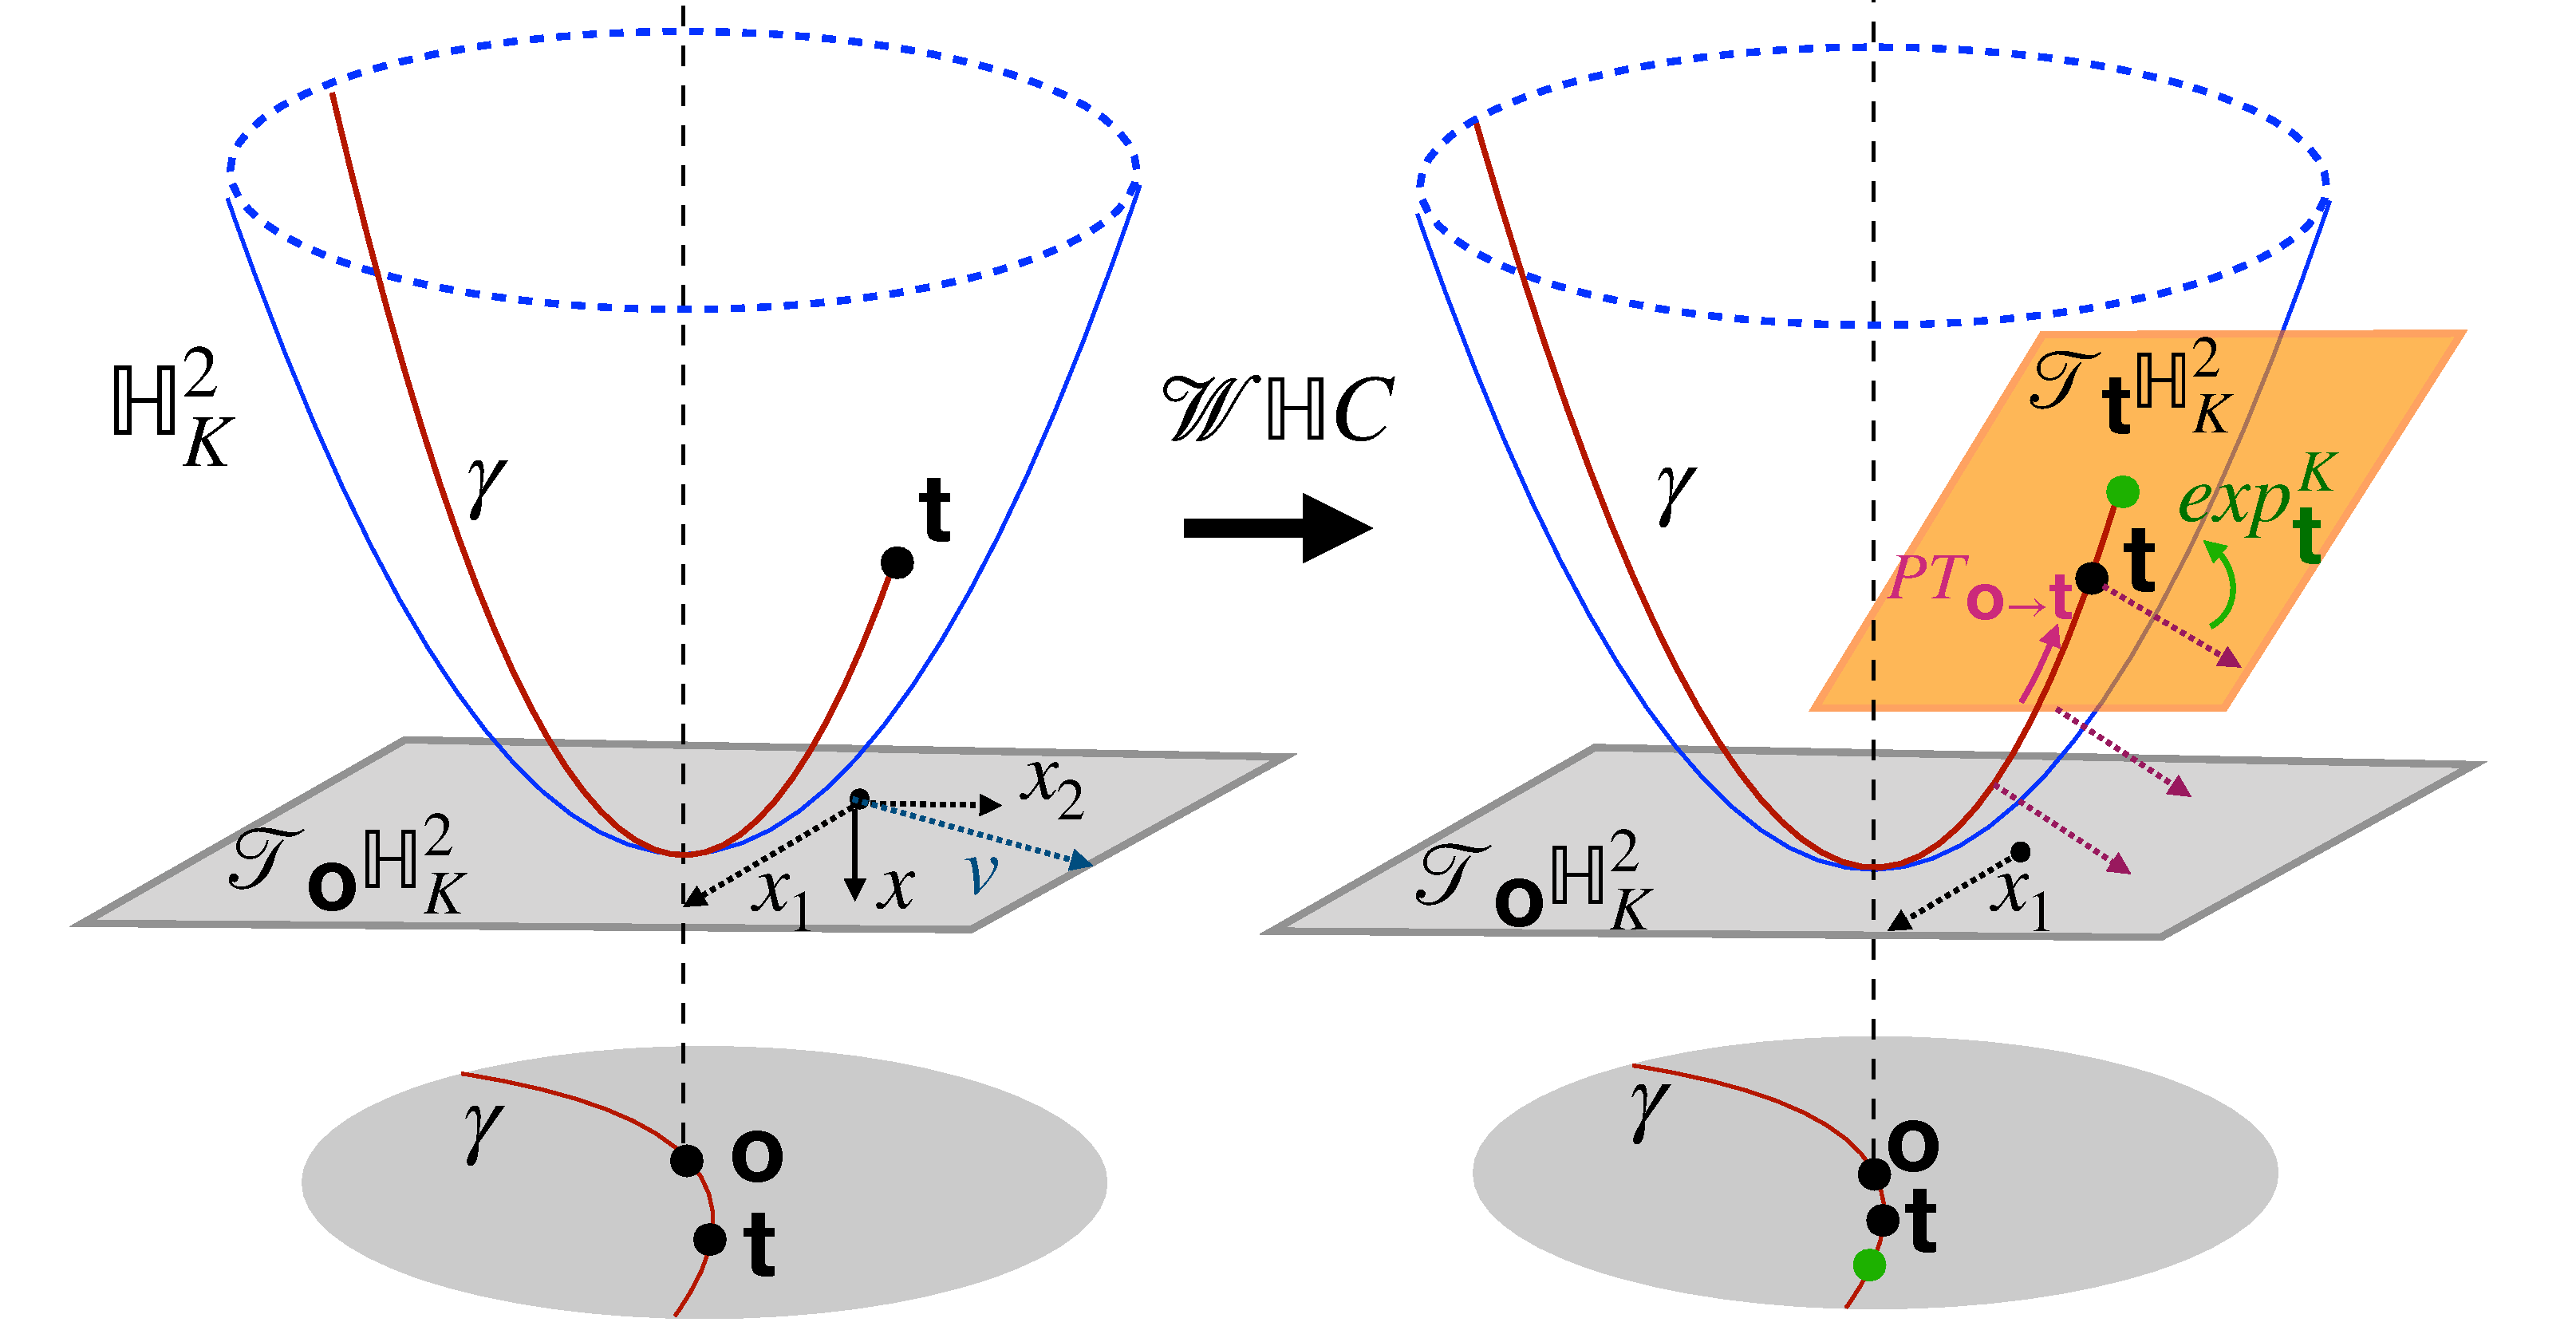
\includegraphics[width=\linewidth]{hyperbolic_flows_arch.pdf}
    \vspace{-5mm}
    \caption{Wrapped Hyperbolic Coupling. The left figure depicts a partitioned input point $x_1:=x_{0:d}$ and $x_2:=x_{d+1:n}$ prior to parallel transport. The right figure depicts the $x_2$ vector after it is transformed, parallel transported, and projected to $\mathbb{H}^n_K$.}
    \vspace{-5pt}
    \label{fig:whc_architecture_diagram}
\end{figure}

\label{wrapped_hyerboloid_coupling_section}
The hyperbolic normalizing flow with $\mathcal{T}C$ layers discussed above operates purely in the tangent space at the origin.
This simplifies the computation of the Jacobian determinant, but anchoring the flow at the origin may hinder its expressive power and its ability to leverage disparate regions of the manifold. 
In this section, we remedy this shortcoming with a new hyperbolic flow that performs translations between tangent spaces via parallel transport. 
%which may lack expressive power. That is to say, by utilizing solely the tangent space at the origin the normalizing flow doesn't utilize different regions of the manifold which may be useful to learning richer and more flexible distributions. One remedy to this fact is to make more explicit use of the manifold by defining different flow operations on different tangent spaces. Specifically, we can define the translation function, $t$, as predicting a tangent space we wish to Parallel transport to rather than simply translating a vector in $\mathcal{T}_{\textbf{o}}\mathbb{H}^n_K$.

We term this transformation {\em Wrapped Hyperboloid Coupling} ($\mathcal{W}\mathbb{H}C$). %which we compose to define a new normalizing flow.
As with the $\mathcal{T}C$ layer, it is a fully invertible transformation $f^{\mathcal{W}\mathbb{H}C}: \mathbb{H}^n_k \to \mathbb{H}^n_k$ with a tractable analytic form for the Jacobian determinant. 
%that learns to transport different partitions of the latent code to different points on the manifold. Critically, the associated change in volume due to $\mathcal{W}\mathbb{H}$-Coupling can be efficiently computed as the Jacobian determinant retains a block triangular structure. 
We employ the coupling strategy previously discussed and partition our input vector into two components: $x_1:=x_{0:d}$ and $x_2:=x_{d+1:n}$.
To define a $\mathcal{W}\mathbb{H}C$ layer we first use the logarithmic map at the origin to transport a point to the tangent space. Let $\tilde{x} = \log_{\textbf{o}}(\mb{x})$ be the point on $\mathcal{T}_{\textbf{o}\mathbb{H}^n_K}$ after the logarithmic map. 
The remainder of the $\mathcal{W}\mathbb{H}C$ layer can be defined as follows;
\begin{align}
\label{wrapped_hyperboloid_coupling_eqn}
\tilde{f}^{\mathcal{W}\mathbb{H}C}(\tilde{x})&=
     \begin{cases}
     \tilde{z}_{1} &= \tilde{x}_{1}  \\
     \tilde{z}_{2} &= \log_{\textbf{o}}\Big( \textnormal{exp}_{t(\tilde{x}_{1})}\big(\textnormal{PT}_{\textbf{o}\to t(\tilde{x}_{1}) }(v)\big)\Big) \nonumber
    \end{cases}\\
    v &= \tilde{x}_{2} \odot \sigma(s(\tilde{x}_{1})) \nonumber \\
    f^{\mathcal{W}\mathbb{H}C}(\mb{x}) &=  \textnormal{exp}_{\textbf{o}}(\tilde{f}^{\mathcal{W}\mathbb{H}C}(\log_{\textbf{o}}(\mb{x}))).
\end{align}
\cut{
\begin{equation}
    \textbf{y} =  \textnormal{exp}_{\textbf{o}}\Big \{b \odot \tilde{x} + (1 - b)\odot \log_{\textbf{o}}\Big( \textnormal{exp}_{t(b \odot \tilde{x})}\big((\textnormal{PT}_{\textbf{o}\to t(b \odot \tilde{x}) }((1-b) \odot \tilde{x} \odot \sigma(s(b \odot \tilde{x})))\big)\Big)\Big \},
\end{equation}
}
Functions $s: \mathcal{T}_{\textbf{o}}\mathbb{H}^{d}_k \to \mathcal{T}_{\textbf{o}}\mathbb{H}^{n-d}_k$ and $t:\mathcal{T}_{\textbf{o}}\mathbb{H}^{d}_k \to \mathbb{H}^n_k$ are taken to be arbitrary neural nets, but the role of $t$ when compared to $\mathcal{T}C$ is vastly different. In particular, the generalization of translation on Riemannian manifolds can be viewed as parallel transport to a different tangent space. Consequently, in Eq.~\ref{wrapped_hyperboloid_coupling_eqn}, the function $t$ predicts a point on the manifold that we wish to parallel transport to.
This greatly increases the flexibility as we are no longer confined to the tangent space at the origin. The logarithmic map is then used to ensure that both $x_1$ and $x_2$ are in the same tangent space before the final exponential map that projects the point to the manifold.

One important consideration in the construction of $t$ is that it should only parallel transport functions of $x_2$. However, the output of $t$ is a point on $\mathbb{H}^n_k$ and without care this can involve elements in $x_1$. To prevent such a scenario we construct the output of $t = [t_0, 0, \dots , 0, t_{d+1}, \dots , t_{n}]$ where elements $t_{d+1:n}$ are used to determine the value of $t_0$ using Eq. \ref{eqn:hyperboloid_projection}, such that it is a point on the manifold and every remaining index is set to zero. Such a construction ensures that only components of any function of $x_2$ are parallel transported as desired. Figure \ref{fig:whc_architecture_diagram} illustrates the transformation performed by the $\mathcal{W}HC$ layer.

\xhdr{Inverse of $\mathcal{W}\mathbb{H}C$}
To invert the flow it is sufficient to show that argument to the final exponential map at the origin itself is invertible. Furthermore, note that $x_1$ undergoes an identity mapping and is trivially invertible. Thus it is sufficient to show that second partition is invertible. That is, we need to show that the following transformation is invertible:
\begin{equation}
     \tilde{z}_{2} = \log_{\textbf{o}}\Big( \textnormal{exp}_{t(\tilde{x}_{1})}\big(\textnormal{PT}_{\textbf{o}\to t(\tilde{x}_{1}) }(v)\big)\Big).
\end{equation}
As discussed in Section \ref{sec:background}, the parallel transport, exponential map, and logarithmic map all have well-defined inverses with closed forms. Thus, the overall transformation is invertible in closed form:
%By equation \ref{eqn:inv_parallel_transport} the inverse of parallel transport is another parallel transport. Also, by definition and equations \ref{eqn:exp_map}-\ref{eqn:log_map} the exponential and logarithmic maps are inverse mappings of each other. Consequently, the overall transformation is invertible and the closed form expression of the inverse is,
\begin{align*}
     \begin{cases}
     \tilde{x}_{1} &= z_{1} \\
     \tilde{x}_{2} &= \Big( \textnormal{PT}_{t(\tilde{z}_{1}) \to \textbf{o} }(\log_{\tilde{y}_{1}}( \textnormal{exp}_{\textbf{o}}(\tilde{z}_{2}))\Big) \odot \sigma(s(\tilde{z}_{1}))^{-1} \\
    \end{cases}
\end{align*}

\xhdr{Properties of $\mathcal{W}\mathbb{H}C$}
To compute the Jacobian determinant of the full transformation in Eq. \ref{wrapped_hyperboloid_coupling_eqn} we proceed by analyzing the effect of $\mathcal{W}\mathbb{H}C$ on valid orthonormal bases for the tangent space at the origin. We state our main result here and provide a sketch of the proof, while the entire proof can be found in Appendix \ref{wrapped_coupling_proof_appendix}. 
\begin{prop}
The Jacobian log-determinant of the function $\tilde{f}^{\mathcal{W}\mathbb{H}C}$ in \eqref{wrapped_hyperboloid_coupling_eqn} is:
\begin{multline}
  \log \left|\textnormal{det}\left(\frac{\partial\mb{y}}{\partial \mb{x}}\right)\right| = \prod_{i=d+1}^n\sigma(s(\tilde{x}_1))_i + \Big(\frac{R \sinh(\frac{||q||_{\mathcal{L}})}{R}}{||q||_{\mathcal{L}}}\Big)^{l} \\
  + \Big(\frac{R\sinh(\frac{||\log_{\textbf{o}}(q)||_{\mathcal{L}}}{R})}{||\log_{\textbf{o}}(q)||_{\mathcal{L}}}\Big)^{-l} \ +  \Big(\frac{R\sinh(\frac{||\tilde{z}||_{\mathcal{L}}}{R})}{||\tilde{z}||_{\mathcal{L}}}\Big)^{n-1}
 \  \\ + \Big(\frac{R\sinh(\frac{||\log_{\textbf{o}}(\textbf{x})||_{\mathcal{L}}}{R})}{||\log_{\textbf{o}}(\textbf{x})||_{\mathcal{L}}}\Big)^{1-n},
\end{multline}
where $\tilde{z} = \textnormal{concat}(\tilde{z}_1, \tilde{z}_2)$, the constant $l = n-d$, $\sigma$ is a pointwise non-linearity 
and $q = \textnormal{PT}_{\textbf{o}\to t(\tilde{x}_1) }(v)$.
\end{prop}
\begin{proofsketch}
We first note that the exponential and logarithmic maps applied at the beginning and end of the $\mathcal{W}\mathbb{H}C$ can be dealt with by appealing to the chain rule and the known log Jacobian determinants for these functions as used in Proposition 1.  
Thus, what remains is the following term: $\left|\textrm{det}\left(\frac{\partial \mb{z}}{\partial \tildex}\right)\right|$. To evaluate this term we rely on the following Lemma:
\begin{lemma}
Let $h : \mc{T}_\mb{o}\mbb{H}^n_k \rightarrow \mc{T}_\mb{o}\mbb{H}^n_k$ be a function from the tangent space at the origin to the tangent space at the origin defined as:
\begin{equation}\label{eq:g2}
h(\tilde{x}) = z = \textnormal{concat}(\tilde{z_1}, \tilde{z_2}).
\end{equation}
Now, define a function $h^* : \mc{T}_\mb{o}\mbb{H}^{n-d} \rightarrow \mc{T}_\mb{o}\mbb{H}^{n-d}$ which acts on the subspace of $\mc{T}_\mb{o}\mbb{H}^{n-d}$ corresponding to the standard basis elements $\mb{e}_{d+1}, ..., \mb{e}_n$ as
\begin{equation}\label{eq:gstar2}
h^*(\tilde{x}_{2}) =   \log_{\mb{o}_{2}}\Big( \textnormal{exp}_{\mb{t}_{2}}\big(\textnormal{PT}_{\mb{o}_{2} \to \mb{t}_{2}}(v)\big)\Big),
\end{equation}
where $\tilde{x}_{2}$ denotes the portion of the vector $\tilde{x}$ corresponding to the standard basis elements $e_{d+1}, ..., e_n$ and $s$ and $t$ are constants (which depend on $\tilde{x}_{1}$).
In Equation \eqref{eq:gstar2}, we use $\mb{o}_{2} \in \mbb{H}^{n-d}$ to denote the vector corresponding to only the dimensions $d+1, ..., n$ and similarly for $\mb{t}_{2}$.
Then we have that
\begin{equation}
    \left|\textnormal{det}\left(\frac{\partial \mb{z}}{\partial \tildex}\right)\right| =    \left|\textnormal{det}\left(\frac{\partial h^*(\tildex_{d+1:n})}{\partial \tildex_{d+1:n})}\right)\right|.
\end{equation}
\end{lemma}
The proof for Lemma 1 is provided in Appendix \ref{wrapped_coupling_proof_appendix}. Using Lemma 1, and the fact that $|\textnormal{det}(\textnormal{PT}_{\textbf{u}\to\textnormal{t}}(v))| = 1$ \cite{nagano2019wrapped} we are left with another composition of functions but on the subspace $\mathcal{T}_{\textbf{o}}\mathbb{H}^{n-d}$. The Jacobian determinant for these functions, are simply that of the logarithmic map, exponential map and the argument to the parallel transport which can be easily computed as $\prod_{i=d+1}^n \sigma(s(\tilde{x}_1))$. 
\end{proofsketch}
The cost of computing the change in volume for one $\mathcal{W}\mathbb{H}C$ layer is $\mathcal{O}(n)$ which is the same as a $\mathcal{T}C$ layer plus the added cost of the two new maps that operate on the lower subspace of basis elements.
